% STATUS: ACTIVE -- second-order gain model (a_x + delta a_x), lambda_f = 1: observability matrix -> weighted line fit -> T_d.
% ======================================================
% Compile: xelatex 0928_obs_second_order.tex   (from reference/eq17_analysis/derivation/)
% Companion of 0927_obs_first_order_v1.tex (same layout). Notation: 0921_5state_noap_simple.tex (teacher chain).
% Sections: 1 model | 2 the matrix | 3 what it shows | 4 solving: weighted line fit | 5 T_d | 6 Kalman filter.
% Figure: fig_noap_descent_o2_td5_td50.png (test_script/scratch/plot_5state_noap_descent_o2_td5_td50.m;
%   runs ladder_ramp16_Td5_lf1_o{1,2}.mat, ladder_ramp16_Td50_lf1_s{1..5}_o{1,2}.mat; descent drawn, 0.5 s holds still in the runs).
% Equations only (derivation-workflow rule 10).
% ======================================================
\documentclass[11pt,a4paper]{ctexart}
\usepackage[fleqn]{amsmath}
\usepackage{amssymb,bm}
\usepackage{graphicx}
\graphicspath{{figures/}}
\setlength{\mathindent}{0pt}
\usepackage{geometry}
\geometry{margin=2.2cm}
\setlength{\parindent}{0pt}
\setlength{\parskip}{0.2em}
\setlength{\abovedisplayskip}{6pt}
\setlength{\belowdisplayskip}{6pt}
\setlength{\abovedisplayshortskip}{6pt}
\setlength{\belowdisplayshortskip}{6pt}
\newcommand{\lc}{\lambda_c}
\newcommand{\hd}[1]{\par\bigskip\noindent\underline{\textbf{#1}}}
\pagestyle{plain}

\begin{document}

\begin{center}\textbf{\large Second-order gain model: observability matrix}\end{center}

%======================================================================
\section{Model}

\hd{State equation}
\[
\begin{aligned}
\delta x_1[k+1] &= \delta x_2[k] \\
\delta x_2[k+1] &= \delta x_3[k] \\
\delta x_3[k+1] &= \lc \cdot \delta x_3[k] - F_{dx}[k]\cdot e_{a_x}[k] + dF_{dx}[k]\cdot e_{\delta a_x}[k] - \varepsilon[k] \\
a_x[k+1] &= a_x[k] + \delta a_x[k] \\
\delta a_x[k+1] &= \delta a_x[k]
\end{aligned}
\]
\[
F_{dx} \approx \big(1 + (1-\lc)d\big)\,\frac{\Delta x_d}{\hat a_x}, \qquad
dF_{dx} = (1-\lc)\textstyle\sum_{i=1}^{d} i\cdot f_{dx}[k-i] \qquad (\text{constant velocity})
\]

\hd{Output equation}
\[
\begin{aligned}
y_1[k] &= \delta x_1[k] + n_x[k], \qquad\qquad\qquad\;\; R_1 = \mathrm{Var}(n_x) \\
y_2[k] &= a_x[k-d] + n_a[k] \approx a_x[k] - d\cdot\delta a_x[k] + n_a[k], \qquad R_2 = \mathrm{Var}(n_a)
\end{aligned}
\]

\hd{Estimation error and output error}
\[
\mathbf{e}[k] = \begin{bmatrix} e_{\delta x_1} & e_{\delta x_2} & e_{\delta x_3} & e_{a_x} & e_{\delta a_x} \end{bmatrix}^T[k]
\]
\[
\begin{aligned}
e_{y_1}[k] &= y_1[k] - \hat y_1[k] = e_{\delta x_1}[k] + n_x[k] \\
e_{y_2}[k] &= y_2[k] - \hat y_2[k] = e_{a_x}[k] - d\cdot e_{\delta a_x}[k] + n_a[k]
\end{aligned}
\]

\hd{Error propagation (no noise)}
\[
\mathbf{e}[k+1] = \mathbf{F}_e[k]\,\mathbf{e}[k], \quad
\mathbf{F}_e[k] =
\begin{bmatrix}
0 & 1 & 0 & 0 & 0 \\
0 & 0 & 1 & 0 & 0 \\
0 & 0 & \lc & -F_{dx}[k] & dF_{dx}[k] \\
0 & 0 & 0 & 1 & 1 \\
0 & 0 & 0 & 0 & 1
\end{bmatrix}
\]
\[
\begin{bmatrix} e_{y_1}[k] \\ e_{y_2}[k] \end{bmatrix} = \mathbf{H}\,\mathbf{e}[k], \quad
\mathbf{H} =
\begin{bmatrix}
1 & 0 & 0 & 0 & 0 \\
0 & 0 & 0 & 1 & -d
\end{bmatrix}
\]

%======================================================================
\section{Observability matrix}

\hd{Errors at step $k_0$, output errors $j$ steps later}
\[
\begin{bmatrix} e_{y_1}[k_0+j] \\ e_{y_2}[k_0+j] \end{bmatrix}
= \mathbf{H}\,\mathbf{F}_e[k_0+j-1]\cdots\mathbf{F}_e[k_0]\;\mathbf{e}[k_0]
\]

\hd{The gain block moves as a line}
\[
e_{a_x}[k_0+j] = e_{a_x}[k_0] + j\cdot e_{\delta a_x}[k_0], \qquad e_{\delta a_x}[k_0+j] = e_{\delta a_x}[k_0]
\]

\hd{The matrix (columns $e_{\delta x_1}, e_{\delta x_2}, e_{\delta x_3}, e_{a_x}, e_{\delta a_x}$ at $k_0$)}
\[
\begin{aligned}
y_2,\ j \ge 0:&\quad [\,0 \;\; 0 \;\; 0 \;\; 1 \;\; j-d\,] \\
y_1,\ j = 0, 1, 2:&\quad [\,1\;0\;0\;0\;0\,],\;\; [\,0\;1\;0\;0\;0\,],\;\; [\,0\;0\;1\;0\;0\,] \\
y_1,\ j \ge 3:&\quad \Big[\,0 \;\; 0 \;\; \lc^{\,j-2} \;\; -\textstyle\sum_{i=0}^{j-3}\lc^{\,j-3-i}F_{dx}[k_0+i] \;\;
\textstyle\sum_{i=0}^{j-3}\lc^{\,j-3-i}\big(dF_{dx}[k_0+i] - i\,F_{dx}[k_0+i]\big)\,\Big]
\end{aligned}
\]

\hd{The gain columns ($F_{dx}$ constant, $j$ large)}
\[
\begin{aligned}
e_{y_2}[k_0+j]\Big|_{\text{gain}} &= 1\cdot\big(e_{a_x}[k_0] + (j - d)\,e_{\delta a_x}[k_0]\big) \\
e_{y_1}[k_0+j]\Big|_{\text{gain}} &\approx -\frac{F_{dx}}{1-\lc}\,\big(e_{a_x}[k_0] + (j - j_1)\,e_{\delta a_x}[k_0]\big), \qquad
j_1 = 3 + \frac{\lc}{1-\lc} + \frac{dF_{dx}}{F_{dx}}
\end{aligned}
\]

%======================================================================
\section{What the matrix shows}

\hd{Every row reads the gain error at one moment on a straight line}
\[
e_{a_x}[k_0] + \tau\,e_{\delta a_x}[k_0] = e_{a_x}[k_0+\tau], \qquad
\tau = j - d \;(y_2), \qquad \tau = j - j_1 \;(y_1)
\]

\hd{Speed enters only the $y_1$ factor}
\[
y_2 \text{ factor} = 1, \qquad
y_1 \text{ factor} = -\frac{F_{dx}}{1-\lc} \propto \frac{\Delta x_d}{\hat a_x}, \qquad
\Delta x_d = \frac{(h_0 - h_b)\,R}{T_d/T_s}
\]

%======================================================================
\clearpage
\section{Solving the matrix equation: weighted line fit}

\hd{4.1 Each row as a reading of the gain at time $k_0+\tau_j$ ($y_1$ rows divided by their factor)}
\[
z_j = e_{a_x}[k_0] + \tau_j\,e_{\delta a_x}[k_0] + \text{noise}_j, \qquad
w_j = \frac{1}{\mathrm{Var}(\text{noise}_j)} = \frac{1}{R_2} \;(y_2), \quad \frac{1}{R_1}\Big(\frac{F_{dx}}{1-\lc}\Big)^{2} \;(y_1)
\]

\hd{4.2 Two unknowns that fit every row best}
\[
\begin{aligned}
\text{minimize}\quad & \sum_j w_j\big(z_j - e_{a_x}[k_0] - \tau_j\,e_{\delta a_x}[k_0]\big)^2 \\
\frac{\partial}{\partial e_{a_x}},\;\frac{\partial}{\partial e_{\delta a_x}} = 0:\quad &
\begin{bmatrix} \sum_j w_j & \sum_j w_j\,\tau_j \\ \sum_j w_j\,\tau_j & \sum_j w_j\,\tau_j^2 \end{bmatrix}
\begin{bmatrix} \hat e_{a_x}[k_0] \\ \hat e_{\delta a_x}[k_0] \end{bmatrix}
= \begin{bmatrix} \sum_j w_j\,z_j \\ \sum_j w_j\,\tau_j\,z_j \end{bmatrix}
\end{aligned}
\]

\hd{4.3 Back to the gain: a straight line through the true gains}
\[
\begin{aligned}
&z_j = a_x[k_0+\tau_j] - \big(\hat a_x[k_0] + \tau_j\,\delta\hat a_x[k_0]\big) + \text{noise}_j \\
&\hat a_x[k_0+N] = A + B\,N, \qquad (A, B) = \arg\min_{A,B}\;\sum_j w_j\big(a_x[k_0+\tau_j] - A - B\,\tau_j\big)^2 \\
&e_{a_x}[k_0+N] = a_x[k_0+N] - \big(A + B\,N\big)
\end{aligned}
\]

%======================================================================
\section{$T_d$}

\hd{5.1 Constant velocity: step number and height are the same axis}
\[
h_d[k_0+\tau] = h_0 - \tau\,\Delta h_d, \qquad \Delta h_d = \frac{(h_0 - h_b)\,T_s}{T_d}
\;\;\Rightarrow\;\;
A + B\,\tau = A + \frac{B}{\Delta h_d}\big(h_0 - h_d\big)
\]

\hd{5.2 The same fit written over height}
\[
\sum_j w_j\big(a_x(h_d[j]) - A' - B'\,h_d[j]\big)^2
= \sum_{\text{bands}} \big(\text{steps in band}\big)\cdot\big(w \text{ per step}\big)\cdot\big(a_x - A' - B'\,h_d\big)^2
\]
\[
\text{steps in band} \propto T_d \;(\text{every band}), \qquad
w \text{ per step} = \underbrace{\frac{1}{R_2}}_{\text{no } T_d} + \underbrace{\frac{1}{R_1}\Big(\frac{F_{dx}}{1-\lc}\Big)^{2}}_{\propto\,1/T_d^2}
\]

\hd{5.3 Result}
\[
\begin{aligned}
y_2 \text{ only:}&\quad \text{objective} \propto T_d \;\Rightarrow\; (A', B') \text{ and } \hat a_x \text{ at } h_b \text{ independent of } T_d \\
y_1 \text{ added:}&\quad \text{weight near the wall} \propto 1/T_d \;\Rightarrow\; \text{line pulled less towards the wall as } T_d \text{ grows}
\end{aligned}
\]

%======================================================================
\section{Kalman filter}

\hd{Gain block, $\mathbf{Q} = 0$, information form}
\[
\begin{aligned}
\mathbf{F}_a &= \begin{bmatrix} 1 & 1 \\ 0 & 1 \end{bmatrix}, \qquad
\big(\mathbf{P}^f[k]\big)^{-1} = \mathbf{F}_a^{-T}\,\mathbf{P}^{-1}[k-1]\,\mathbf{F}_a^{-1} \qquad (\text{old rows moved to step } k) \\
\mathbf{P}^{-1}[k] &= \big(\mathbf{P}^f[k]\big)^{-1} + w_k \begin{bmatrix} 1 \\ -d \end{bmatrix}\begin{bmatrix} 1 & -d \end{bmatrix} \qquad (\text{this step's row added}) \\
\mathbf{P}^{-1}[k] &= \text{the } 2\times 2 \text{ matrix of 4.2, all rows up to step } k \;\Rightarrow\; \hat a_x[k] = \text{the line of 4.3 at step } k
\end{aligned}
\]

\clearpage
\section*{Descent only, $T_d = 5$ s vs $50$ s: filter $\hat a_x$ (blue) vs the weighted line fit of 4.3 (green dashed)}
\begin{center}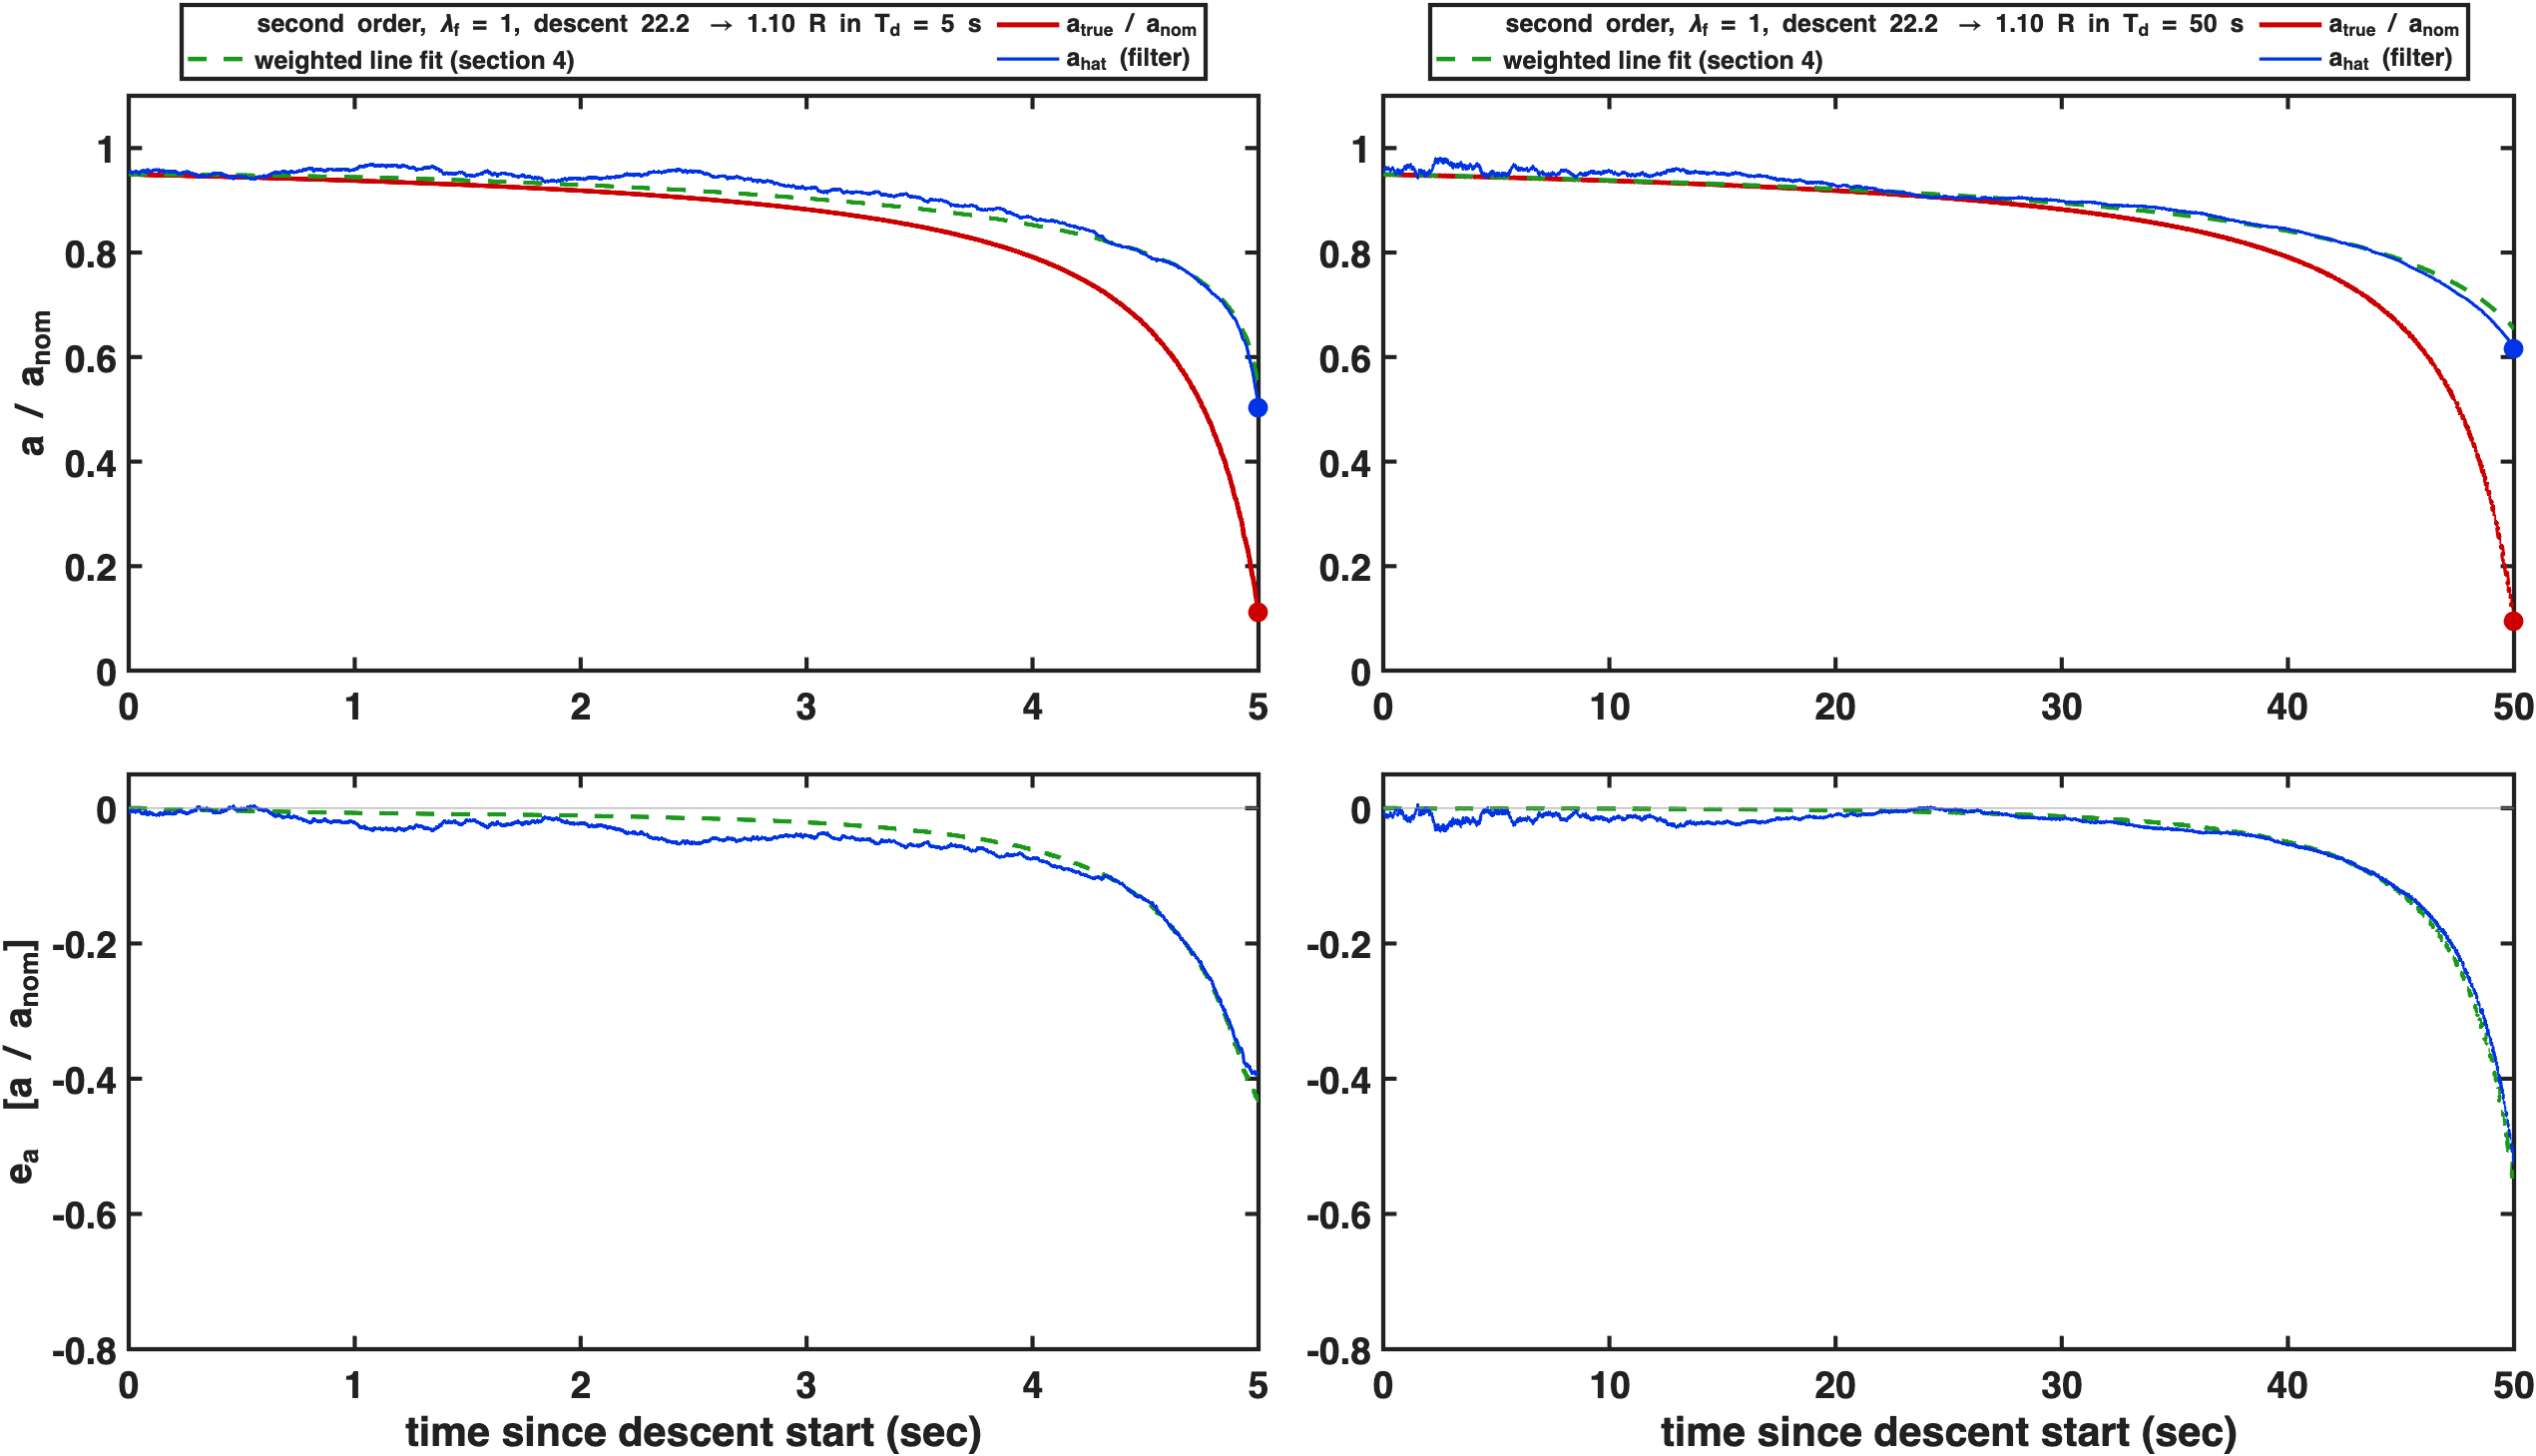
\includegraphics[width=\textwidth]{fig_noap_descent_o2_td5_td50.png}\end{center}

\end{document}
